\documentclass[letter,12pt]{article}
\usepackage[paperheight=27.94cm,paperwidth=21.59cm,bindingoffset=0in,left=3cm,right=2.0cm, top=3.5cm,bottom=2.5cm, headheight=200pt, headsep=1.0\baselineskip]{geometry}
\usepackage{graphicx,lastpage}
\graphicspath{{./}}
\usepackage{upgreek}
\usepackage{censor}
\usepackage[spanish,es-tabla]{babel}
\usepackage{pdfpages}
\usepackage{tabularx}
\usepackage{graphicx}
\usepackage{adjustbox}
\usepackage{xcolor}
\usepackage{colortbl}
\usepackage{rotating}
\usepackage{multirow}
\usepackage[utf8]{inputenc}
\usepackage{float}
\usepackage{hyperref}
\renewcommand{\tablename}{Tabla}
\usepackage{fancyhdr}
\pagestyle{fancy}
%
\begin{document}
%
   \title{\Huge{Informe Laboratorio 2}}
   \author{\textbf{Sección 1} \\  \\Alumno Maximiliano Solorza \\ e-mail: maximiliano.solorza@mail.udp.cl}

   \date{Septiembre de 2026}
   \maketitle

   \tableofcontents

  \newpage

\section*{Blindaje del entorno previo al laboratorio}
\addcontentsline{toc}{section}{Blindaje del entorno previo al laboratorio}

Dado que DVWA es, por diseño, una aplicación \emph{deliberadamente vulnerable} (``\emph{damn vulnerable}''), y que el laboratorio se ejecuta sobre un computador personal con información sensible, previo a levantar el servicio se aplicó un conjunto de medidas de aislamiento (\emph{hardening}) sobre el entorno. El entorno de trabajo es \textbf{Kali Linux corriendo sobre WSL2} (WSL v2.6.2) en Windows~11, con la red de WSL en modo \textbf{NAT} (el modo más aislado; se descartó explícitamente el modo \texttt{mirrored} porque expondría los puertos a la LAN).

\subsection*{Modelo de amenaza}
\addcontentsline{toc}{subsection}{Modelo de amenaza}
DVWA no ataca al equipo por sí misma: es un servidor web que solo resulta peligroso si \textbf{un tercero logra alcanzarlo} por la red y lo explota. Como en este laboratorio el atacante es el propio operador (Burp/cURL/Hydra contra su \texttt{localhost}), el riesgo real se concentra en tres puntos concretos, cada uno con su mitigación:

\begin{enumerate}
    \item \textbf{Exposición de red:} que el puerto de DVWA quede escuchando en \texttt{0.0.0.0} y sea alcanzable desde la LAN/WiFi. \textit{Mitigación:} publicar el servicio únicamente en \texttt{127.0.0.1}.
    \item \textbf{Acceso al disco de Windows:} por defecto WSL monta todo el disco \texttt{C:} en \texttt{/mnt/c} con lectura/escritura, de modo que cualquier proceso dentro de Kali (o un contenedor mal configurado) podría leer o modificar los archivos personales del host. \textit{Mitigación:} desmontar \texttt{/mnt/c} por completo.
    \item \textbf{Privilegios del contenedor:} imágenes no confiables o contenedores con \texttt{-{}-privileged}/\texttt{-{}-network host}. \textit{Mitigación:} imagen oficial, red \emph{bridge} dedicada y contenedores sin privilegios.
\end{enumerate}

\subsection*{Aislamiento del host Windows (\texttt{.wslconfig} y \texttt{wsl.conf})}
\addcontentsline{toc}{subsection}{Aislamiento del host Windows}
Se endureció la configuración global de WSL2 en el archivo \texttt{C:\textbackslash Users\textbackslash Maxi\textbackslash .wslconfig}:
\begin{verbatim}
[wsl2]
memory=6GB
swap=2GB

# NAT = modo mas aislado (NO usar mirrored: expondria puertos a la LAN)
networkingMode=nat
# Firewall Hyper-V activo para el trafico de la VM WSL
firewall=true
# Permite que SOLO el localhost de Windows alcance servicios de WSL
localhostForwarding=true
\end{verbatim}

Y la configuración interna de la distribución Kali en \texttt{/etc/wsl.conf}, para aislar el host:
\begin{verbatim}
[boot]
systemd=true

[automount]
# NO montar automaticamente el disco C: dentro de Kali
enabled=false
mountFsTab=false

[interop]
# Interop encendido (permite lanzar wsl), pero sin PATH de Windows
enabled=true
appendWindowsPath=false
\end{verbatim}

Ambos cambios se aplicaron reiniciando el subsistema con:
\begin{verbatim}
wsl --shutdown
\end{verbatim}

Tras el reinicio se verificó el aislamiento: \texttt{/mnt/c} ya no aparece montado dentro de Kali (el disco de Windows es inaccesible desde la distribución) y el \texttt{PATH} de Kali quedó libre de binarios de Windows. Para transferir el informe y las capturas se emplea la ruta inversa \texttt{\textbackslash\textbackslash wsl.localhost\textbackslash kali-linux\textbackslash} desde el Explorador de Windows, que no depende del \texttt{automount}.

\subsection*{Instalación endurecida de Docker}
\addcontentsline{toc}{subsection}{Instalación endurecida de Docker}
Se instaló el \emph{Docker Engine} nativo dentro de Kali (no Docker Desktop, que integra con Windows), gestionado por systemd:
\begin{verbatim}
apt-get update
apt-get install -y docker.io          # Docker version 28.5.2
systemctl enable --now docker
usermod -aG docker maxo               # ejecutar docker sin sudo
\end{verbatim}

\begin{figure}[H]
    \centering
    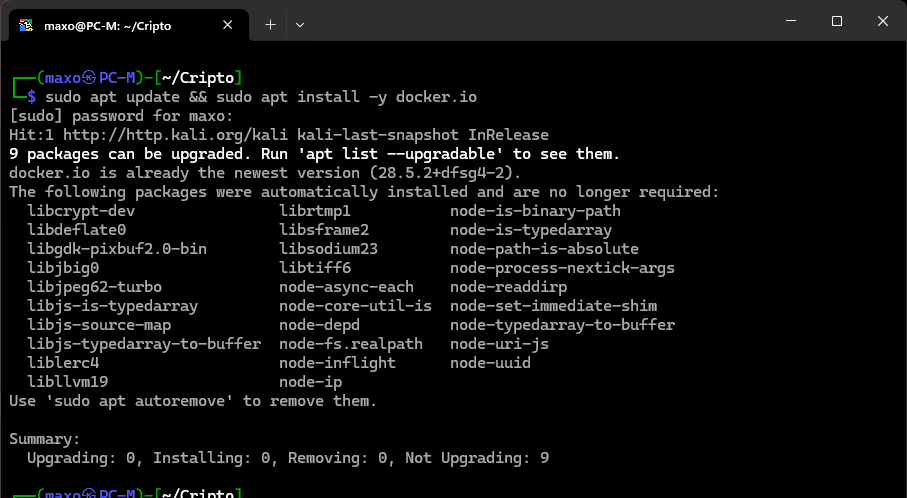
\includegraphics[width=0.9\textwidth]{instalardocker.png}
    \caption{Instalación de Docker Engine (paquete \texttt{docker.io}) en Kali.}
\end{figure}

\begin{figure}[H]
    \centering
    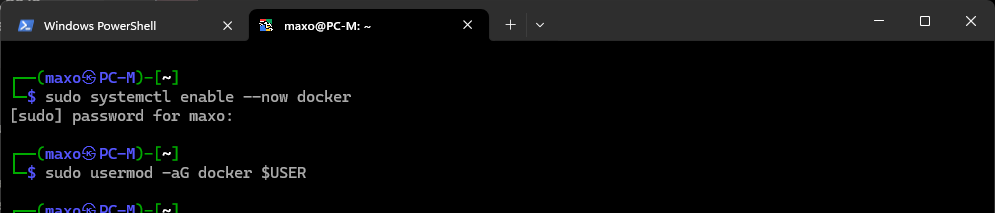
\includegraphics[width=0.9\textwidth]{activardocker.png}
    \caption{Habilitación e inicio del servicio Docker mediante systemd.}
\end{figure}

\begin{figure}[H]
    \centering
    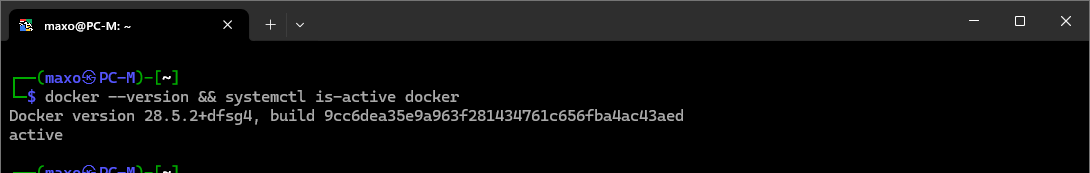
\includegraphics[width=0.9\textwidth]{verificarversionygruo.png}
    \caption{Verificación: Docker 28.5.2 instalado y servicio en estado \texttt{active}.}
\end{figure}

\subsection*{Despliegue aislado de DVWA}
\addcontentsline{toc}{subsection}{Despliegue aislado de DVWA}
El servicio se desplegó sobre una \textbf{red bridge dedicada}, con la base de datos \textbf{sin puerto publicado} (solo accesible dentro de esa red) y DVWA publicada \textbf{exclusivamente en \texttt{127.0.0.1:4280}}, con contenedores sin privilegios adicionales:
\begin{verbatim}
# Red aislada
docker network create dvwa-net

# Base de datos: SIN -p, solo alcanzable dentro de dvwa-net
docker run -d --name dvwa-db --network dvwa-net \
  --security-opt no-new-privileges --restart unless-stopped \
  --memory 512m \
  -e MARIADB_DATABASE=dvwa -e MARIADB_USER=dvwa \
  -e MARIADB_PASSWORD=p@ssw0rd \
  -e MARIADB_ROOT_PASSWORD=<aleatoria> \
  mariadb:lts

# DVWA: publicada SOLO en loopback (nunca 0.0.0.0)
docker run -d --name dvwa --network dvwa-net \
  -p 127.0.0.1:4280:80 \
  --security-opt no-new-privileges --restart unless-stopped \
  --cpus 1 --memory 1g \
  -e DB_SERVER=dvwa-db -e DB_DATABASE=dvwa \
  -e DB_USER=dvwa -e DB_PASSWORD=p@ssw0rd \
  ghcr.io/digininja/dvwa:latest
\end{verbatim}

\begin{figure}[H]
    \centering
    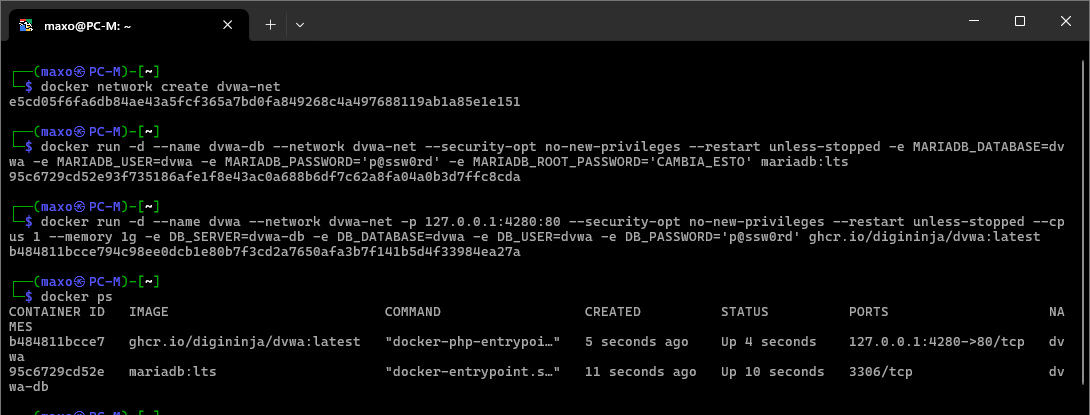
\includegraphics[width=0.9\textwidth]{levantardocker.png}
    \caption{Creación de la red dedicada y levantamiento de los contenedores DVWA y MariaDB.}
\end{figure}

\subsection*{Verificación del aislamiento de red}
\addcontentsline{toc}{subsection}{Verificación del aislamiento de red}
Finalmente se comprobó que el servicio solo escucha en \emph{loopback} y \textbf{no} es alcanzable desde la red:
\begin{verbatim}
# (1) Socket en escucha dentro de Kali -> SOLO 127.0.0.1
$ ss -tlnp | grep 4280
LISTEN 0 4096 127.0.0.1:4280 0.0.0.0:* users:(("docker-proxy",...))

# (2) DVWA responde en loopback
$ curl -s -o /dev/null -w "HTTP %{http_code} -> %{redirect_url}\n" \
       http://127.0.0.1:4280/
HTTP 302 -> http://127.0.0.1:4280/login.php

# (3) Desde la IP de red de Kali (172.25.x.x) -> RECHAZADO
$ curl -s -m 4 http://172.25.189.67:4280/
HTTP 000   (sin respuesta: solo loopback)

# (4) Lado Windows: enlazado a loopback, NO a 0.0.0.0
> netstat -ano -p tcp | findstr 4280
TCP 127.0.0.1:4280 0.0.0.0:0 LISTENING
\end{verbatim}

El resultado confirma la postura buscada: DVWA es accesible únicamente desde el \texttt{localhost} de Kali y desde el \texttt{localhost} de Windows (vía \texttt{localhostForwarding}), pero \textbf{invisible para cualquier otra máquina de la red}. Con el entorno blindado se procede al laboratorio propiamente tal.

\newpage

\section{Descripción de actividades}
Utilizando la aplicación web vulnerable DVWA
(Damn Vulnerable Web App - \href{https://github.com/digininja/DVWA}{https://github.com/digininja/DVWA} (Enlaces a un sitio externo.)) realice las siguientes actividades:
\begin{itemize}
    \item Despliegue la aplicación en su equipo utilizando docker. Detalle el procedimiento y explique los parámetros que utilizó.
    \item Utilice Burpsuite (https://portswigger.net/burp/communitydownload (Enlaces a un sitio externo.)) para realizar un ataque de fuerza bruta contra formulario ubicado en vulnerabilities/brute. Explique el proceso y obtenga al menos 2 pares de usuario/contraseña válidos. Muestre las diferencias observadas en burpsuite.
    \item Utilice la herramienta cURL, a partir del código obtenido de inspect elements de su navegador, para realizar un acceso válido y uno inválido al formulario ubicado en vulnerabilities/brute. Indique 4 diferencias entre la página que retorna el acceso válido y la página que retorna un acceso inválido.
    \item Utilice la herramienta Hydra para realizar un ataque de fuerza bruta contra formulario ubicado en vulnerabilities/brute. Explique el proceso y obtenga al menos 2 pares de usuario/contraseña válidos.
    \item Compare los paquetes generados por hydra, burpsuite y cURL. ¿Qué diferencias encontró? ¿Hay forma de detectar a qué herramienta corresponde cada paquete?
\end{itemize}

\section{Desarrollo de actividades según criterio de rúbrica}

\subsection{Levantamiento de docker para correr DVWA (dvwa)}
Para desplegar DVWA se utilizó la imagen oficial mantenida por el autor del proyecto (\texttt{ghcr.io/digininja/dvwa}), acompañada de un contenedor de base de datos \texttt{mariadb:lts}, siguiendo el mismo despliegue endurecido descrito en la sección \emph{Blindaje del entorno}. El procedimiento fue el siguiente:

\begin{enumerate}
    \item Descargar la imagen oficial desde el registro público:
\begin{verbatim}
docker pull ghcr.io/digininja/dvwa:latest
\end{verbatim}
    \item Crear una red \emph{bridge} dedicada y levantar los contenedores (base de datos sin puerto publicado y DVWA publicada solo en loopback):
\begin{verbatim}
docker network create dvwa-net

docker run -d --name dvwa-db --network dvwa-net \
  --security-opt no-new-privileges --restart unless-stopped \
  -e MARIADB_DATABASE=dvwa -e MARIADB_USER=dvwa \
  -e MARIADB_PASSWORD=p@ssw0rd mariadb:lts

docker run -d --name dvwa --network dvwa-net \
  -p 127.0.0.1:4280:80 \
  --security-opt no-new-privileges --restart unless-stopped \
  --cpus 1 --memory 1g \
  -e DB_SERVER=dvwa-db -e DB_DATABASE=dvwa \
  -e DB_USER=dvwa -e DB_PASSWORD=p@ssw0rd \
  ghcr.io/digininja/dvwa:latest
\end{verbatim}
    \item Acceder a la aplicación desde el navegador en \texttt{http://localhost:4280/}.
    \item Iniciar sesión con las credenciales por defecto \texttt{admin / password}.
    \item Presionar el botón \textbf{Create / Reset Database} para inicializar la base de datos MySQL/MariaDB.
    \item En \textbf{DVWA Security} configurar el nivel de seguridad en \textbf{Low}, requisito para que el formulario de \texttt{vulnerabilities/brute} sea vulnerable a fuerza bruta.
\end{enumerate}

\textbf{Explicación de los parámetros utilizados:}
\begin{itemize}
    \item \texttt{docker run}: crea y ejecuta un nuevo contenedor a partir de una imagen.
    \item \texttt{-d} (detached): ejecuta el contenedor en segundo plano.
    \item \texttt{-{}-name}: asigna un nombre fijo al contenedor (\texttt{dvwa}, \texttt{dvwa-db}) para gestionarlo con facilidad.
    \item \texttt{-{}-network dvwa-net}: conecta el contenedor a una red \emph{bridge} dedicada y aislada.
    \item \texttt{-p 127.0.0.1:4280:80}: publica el puerto (redirección) en formato \texttt{IP\_host:puerto\_host:puerto\_contenedor}; al fijar \texttt{127.0.0.1} el servicio solo queda accesible desde \emph{localhost}.
    \item \texttt{-{}-security-opt no-new-privileges}: impide que los procesos del contenedor escalen privilegios.
    \item \texttt{-{}-restart unless-stopped}: reinicia el contenedor automáticamente salvo que se detenga manualmente.
    \item \texttt{-{}-cpus} / \texttt{-{}-memory}: limitan los recursos que el contenedor puede consumir.
    \item \texttt{-e VARIABLE=valor}: define variables de entorno (aquí, los datos de conexión a la base de datos).
    \item \texttt{ghcr.io/digininja/dvwa:latest} / \texttt{mariadb:lts}: nombres de las imágenes que se ejecutan.
\end{itemize}

\begin{figure}[H]
    \centering
    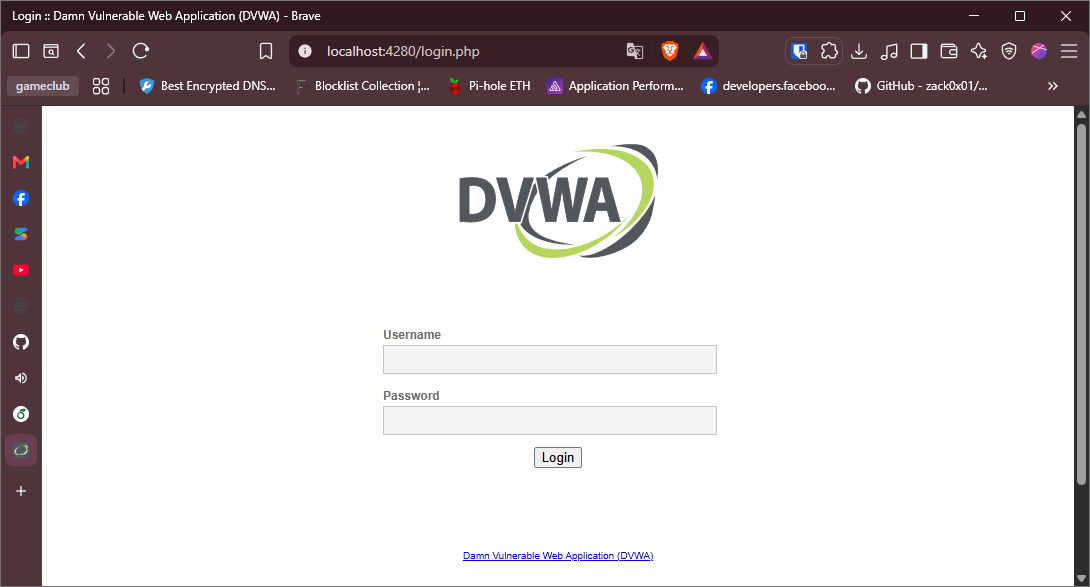
\includegraphics[width=0.9\textwidth]{loginlocal.png}
    \caption{Acceso a DVWA en \texttt{http://localhost:4280} con las credenciales por defecto \texttt{admin/password}.}
\end{figure}

\begin{figure}[H]
    \centering
    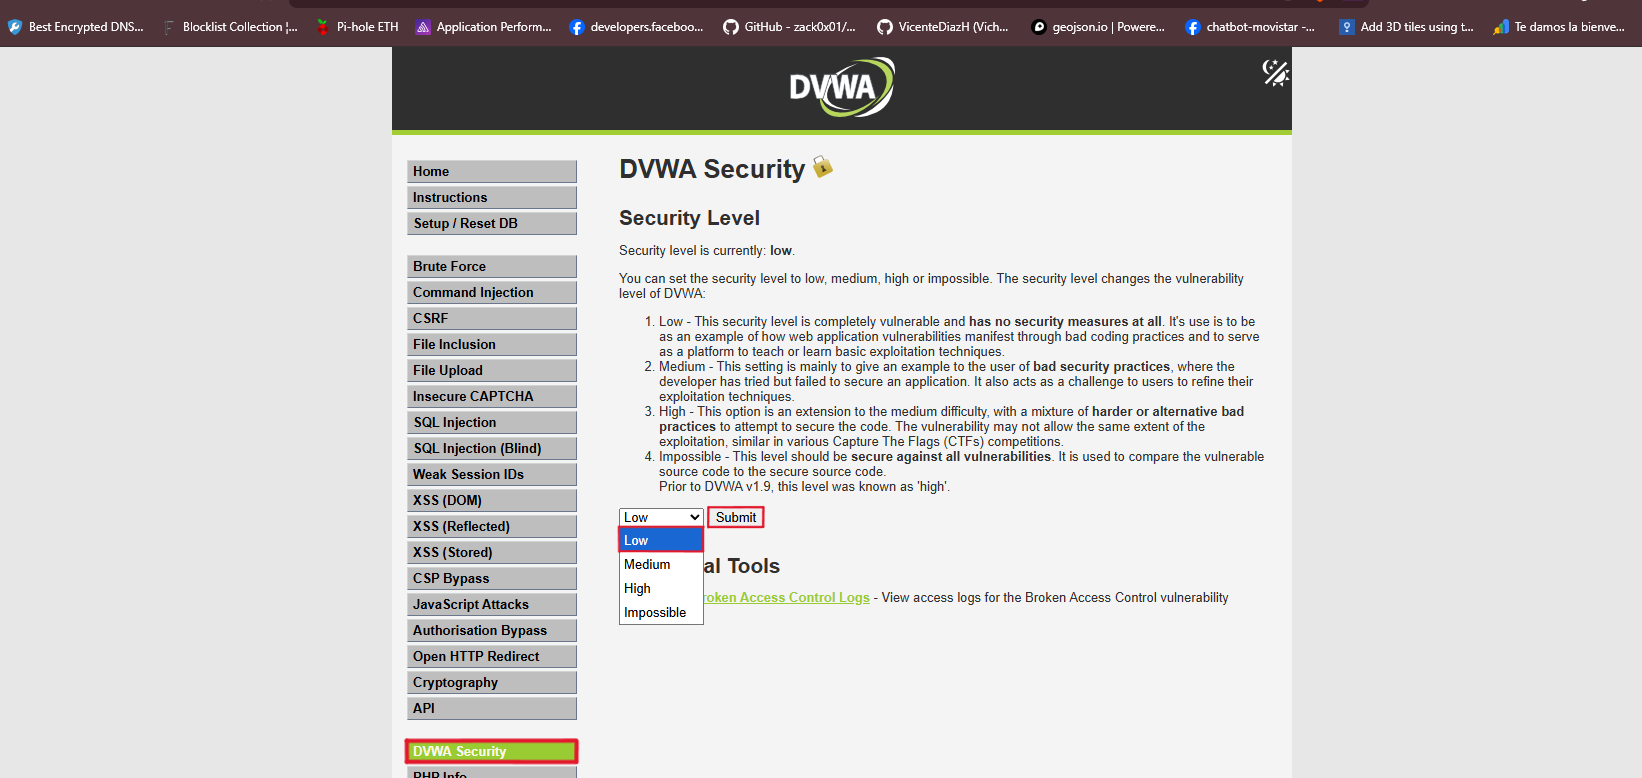
\includegraphics[width=0.9\textwidth]{nivelseguridadLOW.png}
    \caption{Configuración del nivel de seguridad de DVWA en \textbf{Low}.}
\end{figure}

\subsection{Redirección de puertos en docker (dvwa)}
La redirección de puertos se controla con el flag \texttt{-p [IP\_host:]puerto\_host:puerto\_contenedor}. DVWA corre Apache escuchando internamente en el puerto \textbf{80} del contenedor; con \texttt{-p 127.0.0.1:4280:80} ese puerto interno se expone en el puerto \textbf{4280} de la máquina anfitriona, pero \textbf{únicamente en la interfaz de loopback} (\texttt{127.0.0.1}), permitiendo el acceso vía \texttt{http://localhost:4280/} y evitando que el servicio quede expuesto a la red local.

Este detalle es clave desde el punto de vista de seguridad: si se hubiese usado \texttt{-p 4280:80} (o \texttt{-p 80:80}), Docker enlazaría el puerto en \texttt{0.0.0.0}, es decir en \emph{todas} las interfaces, y DVWA sería alcanzable desde cualquier equipo de la LAN, lo cual es inaceptable para una aplicación deliberadamente vulnerable.

Si el puerto elegido estuviera ocupado, basta con cambiar el puerto del host manteniendo el enlace a loopback, por ejemplo \texttt{-p 127.0.0.1:8080:80}, quedando disponible en \texttt{http://localhost:8080/}; internamente el contenedor sigue usando el puerto 80.

La redirección activa puede verificarse con \texttt{docker ps}, que en la columna \texttt{PORTS} muestra el mapeo, en este caso: \texttt{127.0.0.1:4280->80/tcp} (nótese el enlace a loopback y no a \texttt{0.0.0.0}).

\subsection{Obtención de consulta a replicar (burp)}
Burp Suite Community se ejecutó dentro de Kali. Se utilizó su navegador embebido (\textbf{Proxy $\rightarrow$ Open browser}), que ya viene configurado para pasar el tráfico por el proxy de Burp en \texttt{127.0.0.1:8080}.

\begin{figure}[H]
    \centering
    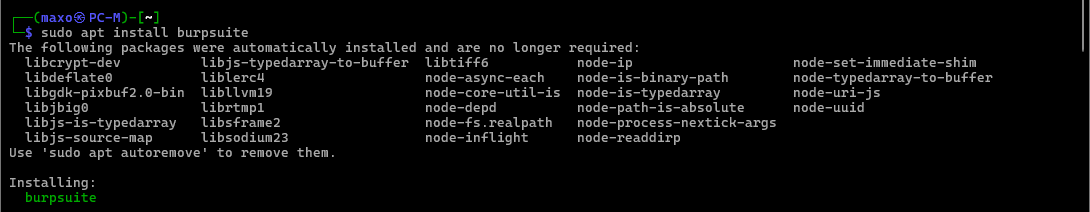
\includegraphics[width=0.7\textwidth]{instalarburpsuit.png}
    \caption{Instalación/inicio de Burp Suite Community en Kali.}
\end{figure}

El formulario objetivo es \texttt{Vulnerabilities $\rightarrow$ Brute Force} de DVWA:

\begin{figure}[H]
    \centering
    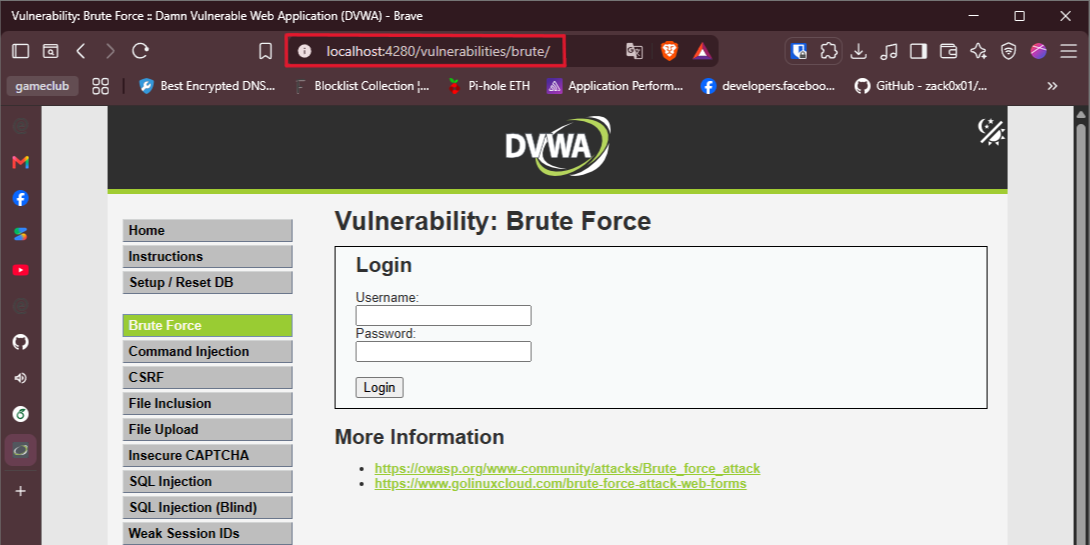
\includegraphics[width=0.9\textwidth]{bruteforce.png}
    \caption{Formulario objetivo: módulo \textit{Brute Force} de DVWA.}
\end{figure}

Con la opción \textbf{Intercept ON} en la pestaña \textit{Proxy}, se envió una solicitud de prueba desde el formulario ingresando un usuario y contraseña cualquiera. Burp capturó la petición HTTP. Como el nivel de seguridad es \textbf{Low}, el formulario envía los datos por método \textbf{GET}, por lo que \textbf{el usuario y la contraseña viajan visibles en la propia URL}:
\begin{verbatim}
GET /vulnerabilities/brute/?username=prueba1&password=canyouseethis_lilpadawan&Login=Login
Host: localhost:4280
Cookie: PHPSESSID=<TU_PHPSESSID>; security=low
\end{verbatim}
Se observan tres parámetros relevantes: \texttt{username}, \texttt{password} y \texttt{Login}. Esta petición interceptada se envió al módulo \textbf{Intruder} con clic derecho $\rightarrow$ \textit{Send to Intruder}.

\begin{figure}[H]
    \centering
    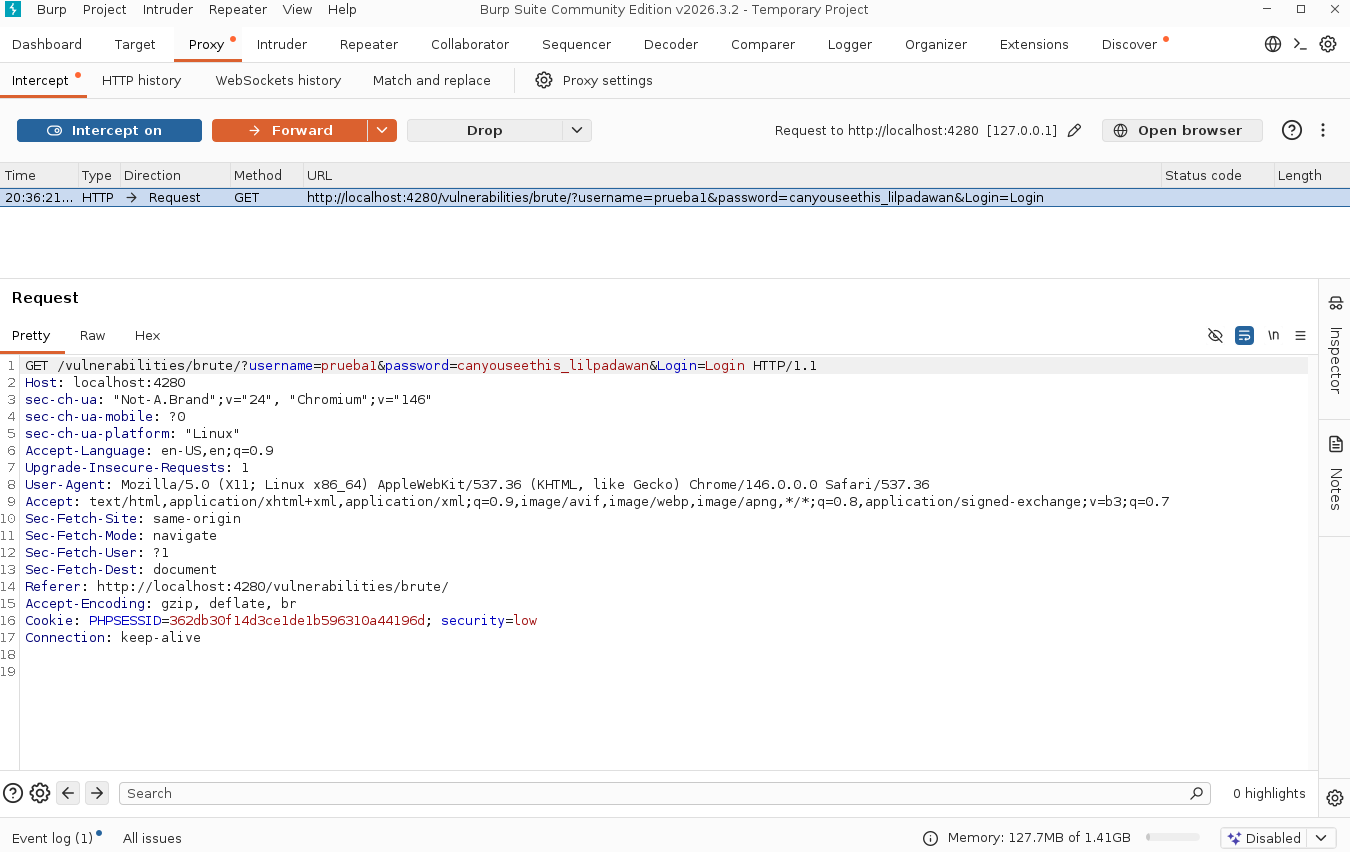
\includegraphics[width=0.95\textwidth]{primerburpsuitloginyclavervisibleenellink.png}
    \caption{Petición interceptada en Burp (Intercept ON): por el método GET, el usuario y la contraseña quedan expuestos en la URL.}
\end{figure}

\subsection{Identificación de campos a modificar (burp)}
Dentro del módulo \textbf{Intruder}, en la pestaña \textit{Positions}, Burp marca automáticamente los parámetros con el símbolo \texttt{\S}. Se limpiaron todas las marcas con \textbf{Clear \S} y luego se marcaron manualmente únicamente los campos \texttt{username} y \texttt{password} como posiciones de payload:
\begin{verbatim}
username=§admin§&password=§test§&Login=Login
\end{verbatim}
Al tener dos posiciones a probar de forma combinada, se seleccionó el tipo de ataque \textbf{Cluster bomb}, que prueba todas las combinaciones posibles de la lista de usuarios contra la lista de contraseñas.

\begin{figure}[H]
    \centering
    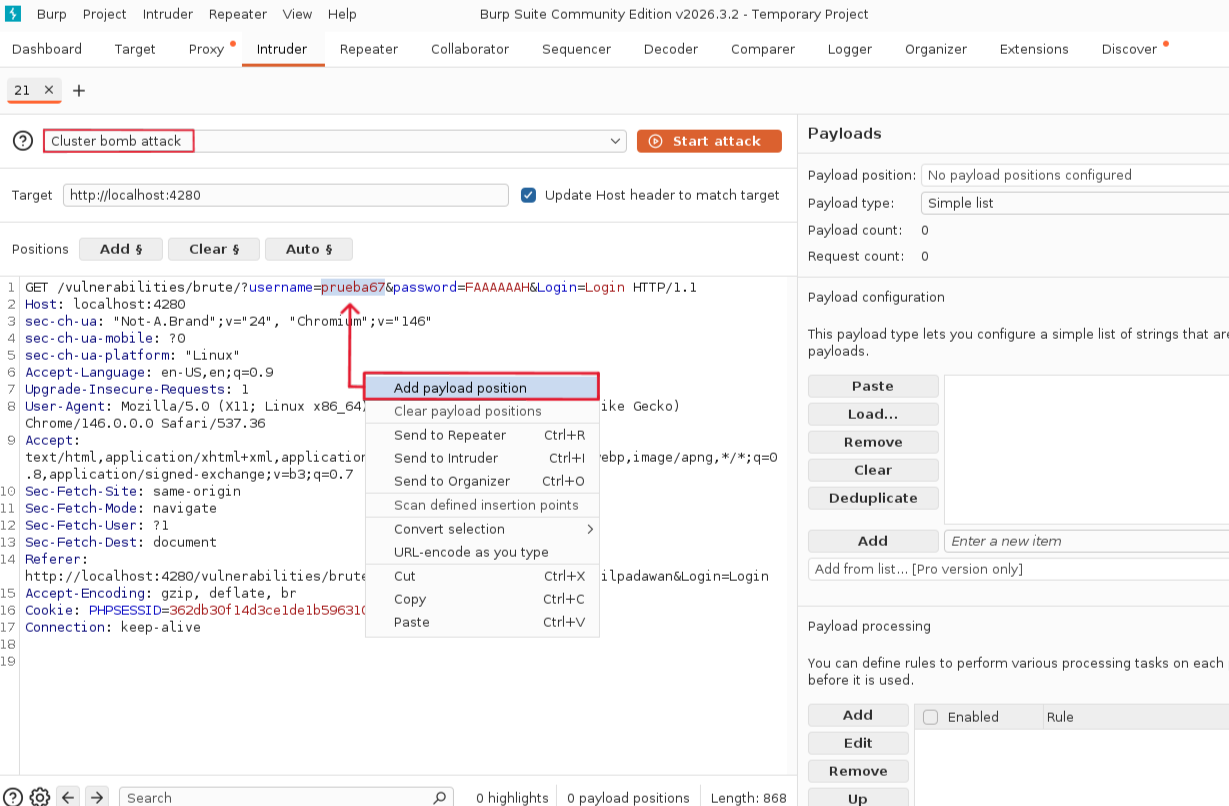
\includegraphics[width=0.95\textwidth]{addpayload.png}
    \caption{Marcado de las posiciones de payload (\texttt{username} y \texttt{password}) y selección del ataque \textbf{Cluster bomb} en Intruder.}
\end{figure}

\subsection{Obtención de diccionarios para el ataque (burp)}
\textbf{Contratiempo con rockyou (gotcha).} Inicialmente se intentó usar el diccionario por defecto de Kali, \texttt{rockyou.txt} (ubicado en \texttt{/usr/share/wordlists/rockyou.txt.gz}, con más de 14 millones de contraseñas). Sin embargo, Burp Intruder \textbf{carga la lista completa en memoria}, por lo que al importar \texttt{rockyou} el consumo de RAM se disparó y la herramienta se volvió inutilizable en el equipo. La solución fue emplear una \textbf{wordlist reducida} de contraseñas comunes (un subconjunto de las más frecuentes, del estilo de las listas ``top-N'' de SecLists), suficiente para el nivel Low y sin impacto en memoria.

\textbf{Enumeración de usuarios (fuga de información).} Un diccionario genérico de contraseñas funciona porque las claves de DVWA son débiles y comunes; en cambio, los \emph{nombres de usuario} (\texttt{gordonb}, \texttt{1337}, \texttt{pablo}, \texttt{smithy}) \textbf{no aparecen en ninguna wordlist genérica}, por ser cuentas propias de la aplicación. Estos se obtuvieron mediante \textbf{enumeración de usuarios}, que constituye en sí misma una vulnerabilidad de fuga de información. Las vías identificadas fueron:
\begin{itemize}
    \item \textbf{Directorio de avatares:} \texttt{/hackable/users/} expone una imagen por usuario cuyo nombre de archivo coincide con el \emph{username} (\texttt{admin.jpg}, \texttt{gordonb.jpg}, \texttt{1337.jpg}, \texttt{pablo.jpg}, \texttt{smithy.jpg}).
    \item \textbf{Documentación / código fuente:} los usuarios por defecto están definidos en el repositorio oficial, en el archivo \texttt{dvwa/includes/DBMS/MySQL.php}.
    \item \textbf{SQL Injection:} el módulo \texttt{vulnerabilities/sqli} permite volcar la tabla \texttt{users} completa (usuarios y sus hashes).
\end{itemize}
Cabe señalar que, en un escenario de caja negra, descubrir usuarios por documentación no es lo más ``realista''; corresponde más bien a una fase previa de \textbf{OSINT / enumeración}. En una auditoría real, los nombres de usuario se obtendrían justamente por fugas de información como las anteriores, y no por fuerza bruta de un diccionario genérico.

Con lo anterior, los diccionarios cargados en Intruder fueron:
\begin{itemize}
    \item \textbf{Payload set 1 (username):} \texttt{admin, gordonb, 1337, pablo, smithy, root, user, test} (usuarios enumerados + genéricos).
    \item \textbf{Payload set 2 (password):} lista reducida de contraseñas comunes: \texttt{password, abc123, charley, letmein, 123456, qwerty, admin, root, test}.
\end{itemize}
Con ambos diccionarios cargados, se inició el ataque con \textbf{Start attack}.

\end{document}
